\documentclass{article}
\usepackage{tikz}
\begin{document}
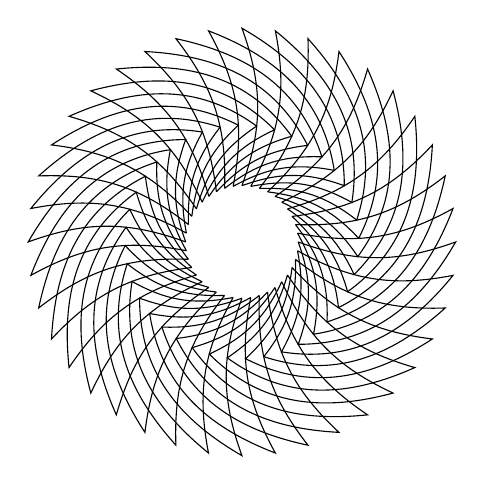
\begin{tikzpicture}
\def\repeatno{40}
\node[inner sep=0.5cm,circle] (base) at (0,0) {};
\foreach \x in {1,2,...,\repeatno}{
\draw[rotate=(\x*360/\repeatno)-90] (base.\x*360/\repeatno) to [in=-70,out=70]  ++(0,2) to [in=90,out=-30] ++(1.3,-2) to [in=20,out=160] +(-1.3,0);
}
\end{tikzpicture}
\end{document}
